%% tl-methoden.tex
\chapter{Methoden}
\label{cha:methoden}

\begin{abstractsec}
  Methoden in Form von klaren Handlungsanweisen erleichtern die Fehlersuche in
  dem Sie den Kopf von Routine entlasten und für das spezielle Problem der
  konkreten Fehlersuche entlasten.
\end{abstractsec}

\begin{notes}
\item Entscheidungsbaum
\end{notes}

\section{Entscheidungsbaum}
\label{sec:entscheidungsbaum}

\begin{abstractsec}
  Eine wichtige Methode ist ein Entscheidungsbaum. Dieser hilft, ein neues
  Problem strukturiert anzugehen und bei komplexen Problemen den jeweils
  nächsten Schritt zu finden.
\end{abstractsec}

\begin{normaltext}
  Wenn ich auf ein neues Problem treffe, versuche ich es so schnell wie
  möglich zu charakterisieren, um die nächsten Schritte zu seiner Behebung
  herauszufinden.
  Dabei helfen mir Entscheidungsbäume. Programmierern ist so etwas
  wahrscheinlich als Programmablaufplan bekannt. Mein grundlegender
  Entscheidungsbaum bei der Fehlersuche sieht immer so aus:

\vspace*{\parskip}
%% hier den Entscheidungsbaum:
%%
%% Ist der Fehler reproduzierbar zu beobachten?
%% nein|  |ja
%%        Funktioniert überhaupt etwas?
%%        nein|  |ja
%%               Funktioniert alles prinzipiell?
%%               nein|  |ja
%%                      Ist es schnell genug?
%%                      nein|  |ja
%%                             Kein Problem, Danke.
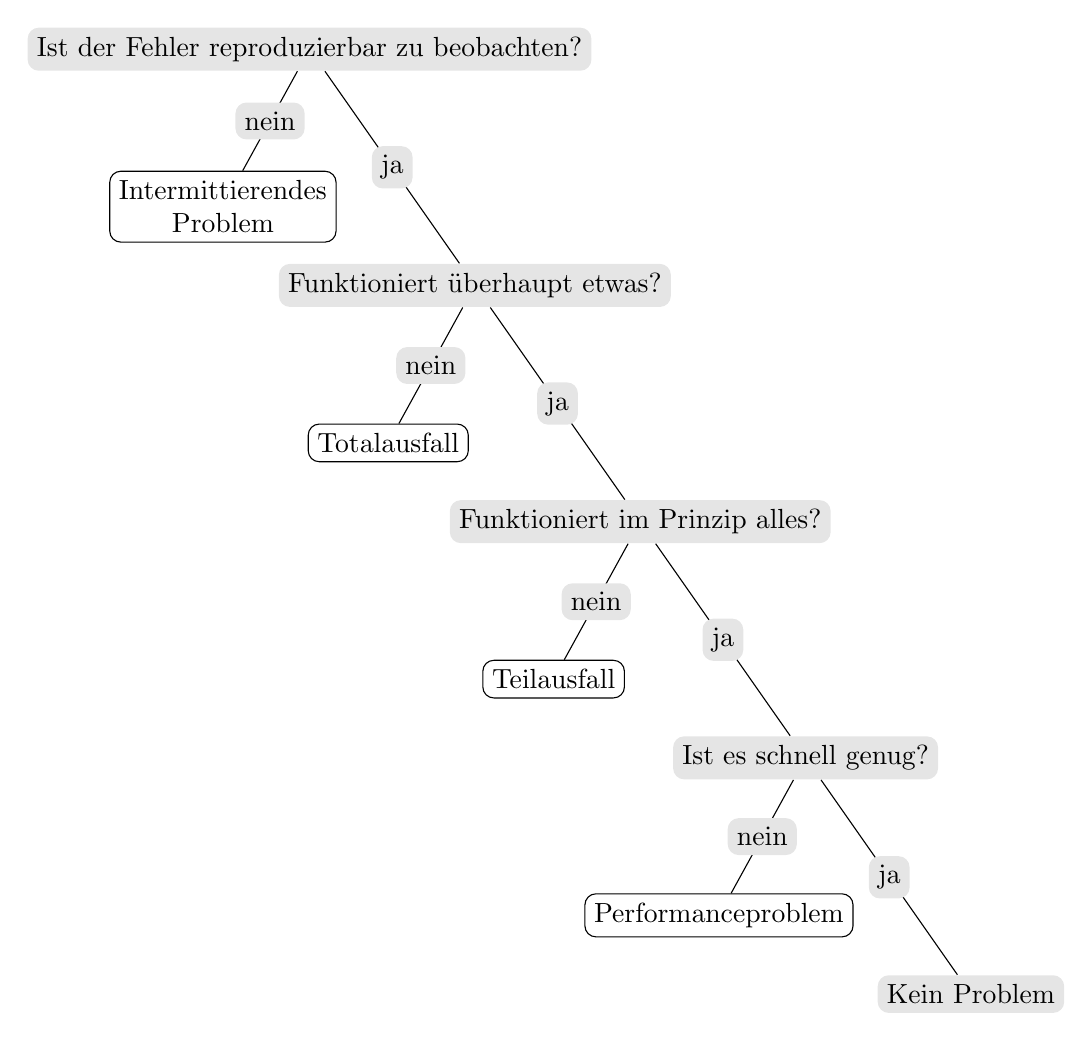
\begin{tikzpicture}
[every node/.style={fill=black!10,rounded corners,align=center},
grow=south, level distance=2cm,
level 1/.style={sibling distance=2.2cm},
level 2/.style={sibling distance=2.2cm},
]
\node{Ist der Fehler reproduzierbar zu beobachten?}
  child{node[draw,fill=white]{Intermittierendes\\Problem}
  edge from parent node[fill=black!10]{nein}}
  child{node at +(1,-1) {Funktioniert überhaupt etwas?}
    child{node[draw,fill=white]{Totalausfall} edge from parent node{nein}}
    child{node at +(1,-1) {Funktioniert im Prinzip alles?}
      child{node[draw,fill=white]{Teilausfall} edge from parent node{nein}}
      child{node at +(1,-1) {Ist es schnell genug?}
        child{node[draw,fill=white]{Performanceproblem}
        edge from parent node{nein}}
        child{node at +(1,-1) {Kein Problem}
        edge from parent node{ja}}
      edge from parent node{ja}}
    edge from parent node{ja}}
  edge from parent node{ja}};
\end{tikzpicture}
\vspace{\parskip}

  Grundsätzlich werde ich nur tätig, wenn eine der Fragen mit nein beantwortet
  wird und habe damit fast alle Probleme abgedeckt.

  Die erste Frage, ob der Fehler reproduzierbar zu beobachten ist, erscheint
  vielleicht trivial, entscheidet aber, ob ich den Fehler überhaupt
  strukturiert eingrenzen oder nur eine Vermutung anstellen kann.
  Wenn ich eine Anfrage via E-Mail bekomme und den Fehler bei mir nicht
  reproduzieren kann, oder wenn mich ein Kunde anruft mit Netzproblemen und
  ich nicht auf sein Netz zugreifen kann, ist damit nicht gemeint. In diesen
  Fällen kann ich, auch wenn ich selbst nicht direkt auf das Problem schauen
  kann, trotzdem anhand des Entscheidungsbaumes zurückfragen. Was ich mit
  dieser Frage ausschließen will, sind intermittierende Probleme. Probleme,
  die auftauchen aber sich der Analyse entziehen. Die scheinbar aus dem Nichts
  kommen und weg sind, sobald ich mich ihnen zuwende. Natürlich kann ich
  die meisten dieser Probleme auch strukturiert bearbeiten. Aber erst muss ich
  sie dingfest machen und gezielt reproduzieren können. Nur dann kann ich
  sicher sein, dass eine vielleicht zufällig gefundene oder erratene Abhilfe
  auch wirklich wirksam ist. In diesen Fällen bleibt mir nichts übrig als
  soviel wie möglich Daten zum Auftreten dieser Fehler zu sammeln und dann mit
  Heuristiken weiter zu sehen.

  Habe ich ein intermittierendes Problem ausgeschlossen, ist meine nächste
  Frage, ob überhaupt noch etwas funktioniert oder es sich um einen
  Totalausfall handelt. Auch diese Frage erscheint vielleicht trivial, aber
  das ist letztendlich der Zweck eines Entscheidungsbaumes: das die richtigen
  (möglichst einfach zu beantwortenden) Fragen im richtigen Moment gestellt
  werden. Manchmal ist es so, dass ein Anwender berichtet, dass eine bestimmte
  Funktion eines Programmes nicht funktioniert und sich irgendwann
  herausstellt, dass der ganze Rechner eingefroren ist und zwar noch den
  letzten Bildschirm zeigt, aber weder auf Tastatur, Maus noch
  Netzwerkzugriffe reagiert. Ein anderes Mal kommt die Meldung, dass das
  Internet nicht geht (Totalausfall) und auf die Bitte ein oder zwei andere
  Websites zu besuchen, sich herausstellt, dass doch nur die eingestellte
  Startseite des Browsers betroffen ist. Darum versuche ich mit dieser Frage
  herauszufinden, ob es sich um einen Totalausfall handelt, der anders
  behandelt werden muß als ein Teilausfall.

  Wenn ich einen Totalausfall ausgeschlossen habe, frage ich als nächstes, ob
  alle für das Problem relevanten Dienste funktionieren. Es erfordert schon
  verhältnismäßig viel Detailkenntnisse zur betreffenden Problemzone, um zu
  entscheiden, ob ein Dienst für das Problem relevant ist oder nicht. Im
  Zweifelsfall kontrolliere ich lieber einen Dienst mehr. Hier geht es vor
  allem darum, einen Überblick zu bekommen, was funktioniert und was nicht und
  dann über Abhängigkeiten der Teilsysteme sich an den oder die Urheber des
  Problems heranzutasten. Dabei gilt es immer im Hinterkopf zu behalten, dass
  es zwar meist einen konkreten Auslöser für ein Problem gibt, oaber oft
  mehrere Ursachen. Eine Möglichkeit, diese Frage zu beantworten, ist zum
  Beispiel verschiedene Funktionen einer Software auszuprobieren, verschiedene
  Netzdienste und Netzziele zu testen. Hierbei kann ein Monitoringsystem wie
  Nagios etc. gute Dienste leisten, wenn es entsprechend aufgesetzt ist.

  Habe ich mich davon überzeugt, dass alle notwendigen Dienste prinzipiell
  funktionieren, kann ich die nächste Frage, ob es schnell genug ist, stellen.
  Diese Frage ist nicht leicht zu beantworten, da jeder seine eigene
  Vorstellung von schnell genug hat. Gibt es SLA, können diese vielleicht bei
  der Beantwortung der Frage helfen. Bei nicht interaktiven Aufgaben, wie
  Datensicherungen, Batchjobs etc. kann man die Gesamtlaufzeit betrachten und
  an Hand dieser entscheiden, ob es schnell genug ist, oder nicht. Bei
  Dateiübertragungen kann man an Hand von Bandbreite, Netzauslastung und
  Übertragungsdauer überschlagen, ob es Performanceprobleme gibt oder nicht.
  Bei interaktiven Programmen oder Netzwerkdiensten zählt meist nur die
  Antwortzeit des Systems, die im Bereich von Sekundenbruchteilen liegen
  sollte. Komme ich zu dem Schluss, dass es sich um ein Performanceproblem
  handelt, gehe ich dieses an. Anderenfalls begründe ich, warum es sich meiner
  Meinung nach um kein Performanceproblem handelt. Dabei kann mir eine
  sogenannte Baseline helfen.

  Alles in allem habe ich mit den vier Fragen dieses Entscheidungsbaumes eine
  Richtschnur, die mir hilft, ein Problem herunterzubrechen und mich dem
  wichtigsten Bereich zu widmen, bevor ich mich in den Details verliere.

  Dabei muss ich den Entscheidungsbaum nicht zwangsläufig von oben nach unten
  verwenden. Wenn mir zum Beispiel ein Netzwerk-Performanceproblem gemeldet
  wird, ist es hilfreich, wenn ich mich zunächst davon überzeuge, dass alle
  Dienste die für das Problem relevant sind, auch funktionieren. Das heißt,
  ich gehe in diesem Fall von unten - dem gemeldeten Performanceproblem -
  einen Schritt nach oben um sicher zu sein, dass meine folgenden Überlegungen
  auf einer gesicherten Basis stehen. Zum Beispiel kann ein ausgefallener
  DNS-Server durch Redundanz zwar kompensiert werden, aber trotzdem zu
  Verzögerungen durch Timeouts führen, die dann als Performanceprobleme
  wahrgenommen werden können.
\end{normaltext}

\section{Bisektion}
\label{sec:bisektion}

\begin{abstractsec}
  Die Bisektion verwende ich bei der Fehlersuche in einem örtlichen oder
  zeitlichen Intervall.
\end{abstractsec}

\begin{normaltext}
  Die Bisektion, auch Intervallhalbierungsverfahren genannt, wird verwendet um
  bei einem Fehler, der auf einer längeren Strecke - zum Beispiel bei einer
  Netzwerkverbindung über mehrere Hops - oder über einen längeren Zeitraum
  auftritt, den Punkt, an dem der Fehler erstmalig auftritt, so schnell wie
  möglich zu ermitteln. Diesen Punkt suche ich, da er mir vermutlich Hinweise
  auf die Ursache geben kann.

  Das Intervall kann örtlich sein - zum Beispiel bei einer Datenübertragung
  über mehrere Hops - oder zeitlich - zum Beispiel, wenn sich der Fehler in
  Logfiles zeigt und ich den Zeitpunkt des ersten Auftretens über viele
  Logdateien hinweg suche.

  Das Verfahren selbst ist sehr einfach. Anstatt das Intervall sequentiell in
  einer Richtung abzuschreiten, wird das Intervall halbiert und von den
  entstehenden Teilintervallen dasjenige untersucht, dessen Grenzen sich
  unterscheiden. Bei diesem Teilintervall fährt man mit der Bisektion fort.

  Wenn ich zum Beispiel einen Rechner in einem weit entfernten Netz zwar via
  Ping erreichen kann, aber zum Beispiel nicht mit Port 25, dann kann ich 
  zunächst untersuchen, ob Datenpakete zu Port 25 beim Sender rauskommen und
  ob sie beim Empfänger ankommen. Kann ich die Datenpakete beim Sender
  nachweisen, aber beim Empfänger nicht, dann suche ich etwa auf der Hälfte
  der Strecke, ob diese Datenpakete nachzuweisen sind. Je nachdem, ob die
  Datenpakete dort auftreten oder nicht, halbiere ich dann die Strecke zum
  Empfänger oder zum Sender. 
\end{normaltext}

%\section{Nicht verrückt machen lassen}
%\label{sec:nicht-verrueckt}

%\begin{abstractsec}
%  sonst kann man nicht klar denken.
%\end{abstractsec}
%\begin{normaltext}
%  Blablabla
%\end{normaltext}

%\subsection{Seiteneffekte}
%\label{sec:seiteneffekte}

%\begin{notes}
%\item Entscheidungsbaum
%\end{notes}

%\section{Heuristiken}
%\label{heuristiken}

%\begin{abstractsec}
%  Wenn gar nichts mehr geht, helfen vielleicht Heuristiken.
%\end{abstractsec}

%\begin{notes}
%\item zeitliche Korrelation
%\end{notes}

%%% Local Variables: 
%%% mode: latex
%%% TeX-master: "arbeit-hauptdatei"
%%% End: 
%%% vim: set sw=2 ts=2 tw=78 et si:
